% CS704 Project 2 -- Deliverable 5: Group report (max 4 pages, due 19 Oct 5pm)
% Compile with pdflatex (Overleaf: works as-is). Submit as project2_group03.pdf.
%
% The only red (\tbd{...}) placeholder left is the author list. Remove the xcolor/\tbd lines
% once it is filled.
\documentclass[conference,a4paper]{IEEEtran}
\usepackage{amsmath}
\usepackage{array}
\usepackage{booktabs}
\usepackage{graphicx}
\usepackage{cite}
\usepackage{xcolor}
\usepackage{tikz}
\usetikzlibrary{positioning,arrows.meta}
\usepackage[hidelinks]{hyperref}
\newcommand{\tbd}[1]{\textcolor{red}{[#1]}}

\begin{document}

\title{Real-Time Step Counting and Heading Estimation on the SensorTile}

\author{\IEEEauthorblockN{Group 3: \tbd{member names and UPIs}}
\IEEEauthorblockA{CS704 Project 2, University of Auckland}}

\maketitle

\begin{abstract}
Satellite positioning does not work reliably inside buildings, so tracking staff in a factory
needs a different approach. In this project we built a pedestrian dead reckoning prototype
for AICorp on the STMicroelectronics SensorTile. The device counts steps, estimates distance
and reports heading in real time, and sends the results to a phone over Bluetooth. Steps are
detected with an adaptive peak and valley method on the magnitude of the acceleration, so the
count does not depend on how the board is worn. Heading comes from a tilt-compensated,
self-calibrating magnetometer combined with the SensorTile's gyroscope, which keeps turns
tracked near steel, where the magnetic field is distorted. The walking direction is either
learnt from the motion of the body or set with a hand gesture, so the board can be carried in
a trouser pocket. In our trials every step on a 44-step route was counted, and on a repeat of
the route the heading on the long straight legs was within 3 degrees of a phone compass.
\end{abstract}

\begin{IEEEkeywords}
pedestrian dead reckoning, step detection, heading estimation, sensor fusion
\end{IEEEkeywords}

\section{Introduction}
AICorp wants to know where its employees are inside a factory, both for safety and so that
help can reach them quickly after an incident. GPS signals are blocked or reflected indoors,
and fitting a building with beacons is expensive, so the brief asks for a wearable device that
tracks a person's step count and orientation by itself. Each group was given a SensorTile kit,
which carries an accelerometer and magnetometer (LSM303AGR) and a gyroscope (LSM6DSM), and the
results are shown in the ST BLE Sensor phone app.

With a step length added, the step count and heading are enough to rebuild a walked path from
a known starting point. This is known as pedestrian dead reckoning (PDR)~\cite{jin2011,tian2016}.
Our device has to stay accurate in a factory, where steel structures and machinery distort the
Earth's magnetic field, and it should work however the worker carries it.

\section{Background}
\subsection{Pedestrian Dead Reckoning}
Integrating acceleration twice to get position drifts within seconds with low-cost MEMS
sensors, unless the sensor is mounted on the foot and corrected every time the foot is flat on
the ground~\cite{jin2011}. Body-worn systems therefore use step-based PDR, where each detected
step moves the position forward by a step length $L_k$ in the current heading $\psi_k$:
\begin{equation}
\mathbf{p}_k=\mathbf{p}_{k-1}+L_k\,[\cos\psi_k,\ \sin\psi_k]^{\mathsf T}.
\end{equation}
The problem then splits into three parts: detecting steps, estimating their length, and
estimating the heading.

\subsection{Step Detection}
Most step detectors look for the periodic peaks that walking produces in the acceleration.
Jin et al.~\cite{jin2011} rotate the acceleration into a world frame and look for a peak
followed by a valley on the vertical axis. Tian et al.~\cite{tian2016} first work out how the
phone is carried (held, swinging or in a pocket) and then apply a threshold to the axis that
suits that mode. Lee et al.~\cite{lee2015} avoid both by using the magnitude of the
acceleration, which does not change with orientation, with thresholds that adapt to the recent
signal. They reported 99.5\% accuracy over seven placements. Brajdic and Harle~\cite{brajdic2013}
compared eight step counters on 130 recordings. Simple windowed peak detection did best, and
they recommend checking the signal's standard deviation so that no steps are counted while the
user stands still. Step length is often estimated with the Weinberg model~\cite{weinberg2002},
which relates it to the fourth root of the acceleration range within the step.

\subsection{Heading Estimation}
Jin et al.~\cite{jin2011} used only an accelerometer and compass, and found that metal cabinets
near the walking path were one of their main sources of heading error. Tian et
al.~\cite{tian2016} integrated the gyroscope instead and learnt the offset between the phone
and the walking direction, but gyroscope drift then became their largest error. Filter-based
methods combine the two. Yuan et al.~\cite{yuan2015} used a quaternion unscented Kalman filter
in which the gyroscope predicts the orientation and the accelerometer and magnetometer correct
it, and achieved a mean heading error below $10^\circ$ with a waist-mounted sensor. Kuang et
al.~\cite{kuang2018} only used the magnetometer while the field was steady. Their heading error
was $2.3^\circ$ RMS with the phone in the hand but $16.6^\circ$ in a pocket.

\begin{table}[!t]
\centering
\footnotesize
\setlength{\tabcolsep}{3pt}
\caption{Approaches in the reviewed literature}
\label{tab:lit}
\begin{tabular}{@{}l>{\raggedright\arraybackslash}p{2.55cm}>{\raggedright\arraybackslash}p{2.35cm}>{\raggedright\arraybackslash}p{1.75cm}@{}}
\toprule
Work & Step detection & Heading & Reported result \\
\midrule
\cite{jin2011} & Peak--valley, vertical axis & Compass, two devices fused & up to 73.7\% less error \\
\cite{tian2016} & Carrying mode, then threshold & Gyroscope, learnt offset & 98.9\% position accuracy \\
\cite{lee2015} & Adaptive thresholds on $|\mathbf{a}|$ & -- & 99.5\% of steps \\
\cite{brajdic2013} & Benchmark of eight methods & -- & median error $<$1.3\% \\
\cite{yuan2015} & -- & Kalman filter, gyro + acc + mag & $<$10$^\circ$ mean \\
\cite{kuang2018} & Peak, Weinberg length & Kalman filter, steady-field mag & 2.3--16.6$^\circ$ RMS \\
\bottomrule
\end{tabular}
\end{table}

\subsection{Implications for This Project}
Table~\ref{tab:lit} summarises these works. Two findings shaped our design. First, adaptive
thresholds on the acceleration magnitude count steps well without knowing how the device is
carried~\cite{lee2015,brajdic2013}. Second, a magnetometer-only heading is cheap but
unreliable near steel, and the usual fix is to combine it with a gyroscope and ignore the
magnetometer when the field looks disturbed~\cite{yuan2015,kuang2018}. Since a factory is full
of steel, we decided to use the SensorTile's gyroscope as well, even though the brief only
mentions the accelerometer and magnetometer.

\section{System Design}
\subsection{Overview}
The firmware runs on the SensorTile's STM32L476 microcontroller. A timer sets a flag every
20\,ms, and the main loop then reads all three sensors over SPI, converts the readings to
physical units and passes them to two independent modules, one for steps and one for heading
(Fig.~\ref{fig:arch}). The results go out in the BLE motion characteristic that the starter
code already used. The accelerometer and magnetometer slots carry the raw data, and the three
gyroscope slots carry the step count, heading and distance, so the ST BLE Sensor app can plot
all of them without any changes.

The accelerometer runs at 50\,Hz with a $\pm4$\,g range in 12-bit mode, which gives a
resolution of 1.95\,mg and leaves headroom for heel strikes. The magnetometer runs at 100\,Hz
with temperature compensation, and the gyroscope at 52\,Hz with a $\pm500$\,dps range. All
three use block data update, so a reading never mixes bytes from two samples. The sensors do
not share the same axes. The gyroscope chip is rotated by $90^\circ$ relative to the
LSM303AGR, and the LSM303AGR's own axes turned out to be mirrored, which we only noticed when
the heading went down instead of up as the board was turned clockwise. The firmware maps all
readings into one right-handed frame before using them.

\begin{figure*}[!t]
\centering
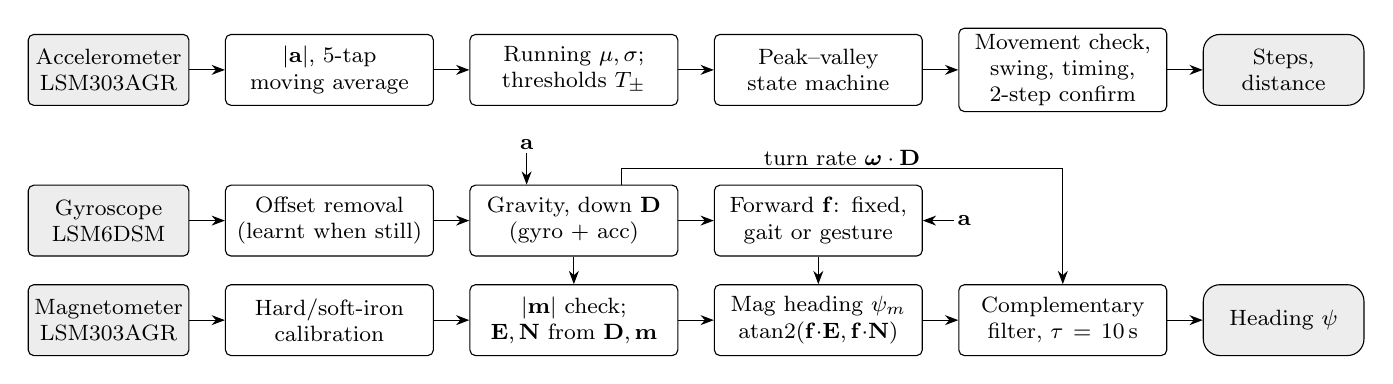
\begin{tikzpicture}[font=\footnotesize, >=Stealth, node distance=3.5mm and 4.5mm,
  blk/.style={draw, rounded corners=2pt, align=center, minimum height=9mm, inner sep=2pt,
              text width=#1},
  blk/.default=25mm,
  io/.style={blk=19mm, fill=black!7},
  res/.style={blk=19mm, fill=black!7, rounded corners=6pt}]
% step-detection path
\node[io] (acc) {Accelerometer\\LSM303AGR};
\node[blk, right=of acc] (s1) {$|\mathbf{a}|$, 5-tap\\moving average};
\node[blk, right=of s1] (s2) {Running $\mu,\sigma$;\\thresholds $T_\pm$};
\node[blk, right=of s2] (s3) {Peak--valley\\state machine};
\node[blk, right=of s3] (s4) {Movement check,\\swing, timing,\\2-step confirm};
\node[res, right=of s4] (o1) {Steps,\\distance};
\draw[->] (acc) -- (s1); \draw[->] (s1) -- (s2); \draw[->] (s2) -- (s3);
\draw[->] (s3) -- (s4); \draw[->] (s4) -- (o1);
% heading path
\node[io, below=10mm of acc] (gyr) {Gyroscope\\LSM6DSM};
\node[io, below=of gyr] (mag) {Magnetometer\\LSM303AGR};
\node[blk, right=of gyr] (h1) {Offset removal\\(learnt when still)};
\node[blk, right=of h1] (h2) {Gravity, down $\mathbf{D}$\\(gyro $+$ acc)};
\node[blk, right=of h2] (fw) {Forward $\mathbf{f}$: fixed,\\gait or gesture};
\node[blk, right=of mag] (h3) {Hard/soft-iron\\calibration};
\node[blk, right=of h3] (h4) {$|\mathbf{m}|$ check;\\$\mathbf{E},\mathbf{N}$ from $\mathbf{D},\mathbf{m}$};
\node[blk, right=of h4] (h5) {Mag heading $\psi_m$\\$\operatorname{atan2}(\mathbf{f}{\cdot}\mathbf{E},\mathbf{f}{\cdot}\mathbf{N})$};
\node[blk, right=of h5] (fu) {Complementary\\filter, $\tau=10$\,s};
\node[res, right=of fu] (o2) {Heading $\psi$};
\draw[->] (gyr) -- (h1); \draw[->] (h1) -- (h2); \draw[->] (h2) -- (fw);
\draw[->] (mag) -- (h3); \draw[->] (h3) -- (h4); \draw[->] (h4) -- (h5);
\draw[->] (h5) -- (fu); \draw[->] (fu) -- (o2);
\draw[->] (h2) -- (h4); \draw[->] (fw) -- (h5);
\draw[<-] ([xshift=-6mm]h2.north) -- ++(0,4mm) node[above, inner sep=1pt] {$\mathbf{a}$};
\draw[<-] (fw.east) -- ++(4mm,0) node[right, inner sep=1pt] {$\mathbf{a}$};
\draw[->] ([xshift=6mm]h2.north) -- ++(0,2mm) -| node[pos=0.25, above, inner sep=1pt]
  {turn rate $\boldsymbol{\omega}\cdot\mathbf{D}$} (fu.north);
\end{tikzpicture}
\caption{Flowchart of the firmware, run once per 20\,ms sample. Top: step detection. Bottom:
heading estimation, where the accelerometer $\mathbf{a}$ also feeds the gravity estimate and the
walking-direction learner.}
\label{fig:arch}
\end{figure*}

\subsection{Step Detection}
Wherever the board is worn, each step produces a rise in acceleration above 1\,g at heel strike
and a dip below 1\,g as the body falls into the next step, and we count one step for each rise
followed by a dip. So that the count does not depend on how the board is worn, the detector
uses the magnitude $|\mathbf{a}|$ rather than a single axis, smoothed with a 5-sample
(100\,ms) moving average.

The thresholds adapt to the walker. A running mean $\mu$ and standard deviation $\sigma$ of the
smoothed signal are kept with exponential moving averages over about one second, and the upper
and lower thresholds are
\begin{equation}
T_\pm=\mu\pm\max(0.3\,\sigma,\ 35\,\text{mg}).
\end{equation}
The 35\,mg floor stops the thresholds from sinking into the sensor noise when the signal is
quiet. A small state machine then records the highest point above $T_+$ and the lowest point
after it below $T_-$. A peak with no valley within 1\,s is thrown away.

A completed peak and valley only count as a step if three conditions hold. The standard
deviation must be above 40\,mg, which shows that the person is moving~\cite{brajdic2013}. The
swing from peak to valley must be at least 120\,mg. The step must also not come too soon after
the previous one: the minimum gap is half the recent average step interval, and never less
than 250\,ms, which stops a double bump within one step from being counted twice. Counting only
starts after two valid steps in a row, so a single knock or sitting down adds nothing, and a
pause longer than 2\,s ends the walk. Every rejected cycle is printed over UART with the reason
it failed, which made tuning much easier.

Each step's length is estimated with the Weinberg model~\cite{weinberg2002},
$L=K\sqrt[4]{a_{\max}-a_{\min}}$, using the peak-to-valley swing in m/s\textsuperscript{2} and
$K=0.45$. The distance is the sum of the step lengths.

\subsection{Heading Estimation}
Heading is reported in degrees clockwise from magnetic north. It comes from the corrected
magnetometer, while the gyroscope follows turns and carries it through distorted areas.

\subsubsection{Gravity}
Tilt correction needs to know which way is down. The accelerometer gives this when the board is
still, but while walking it also measures the body's motion. Each sample, the firmware rotates
its previous gravity estimate using the gyroscope and then moves it 2\% of the way towards the
accelerometer reading, which averages the walking motion out over about a second. The downward
direction $\mathbf{D}$ is the normalised, reversed gravity vector.

\subsubsection{Calibration}
The board's battery and circuitry add a constant offset to the magnetometer reading (hard iron,
about 350\,mG on the Z axis of our board) and scale each axis slightly differently (soft
iron)~\cite{an4825}. After power-up the user turns the board so that each face points up in
turn, while the firmware records the minimum and maximum on each axis. The middle of each range
gives the offset, and each axis is rescaled so that all three ranges have the same radius $R$.
The calibration is used once every axis has swung by at least 800\,mG; Auckland's field is
about 550\,mG, so a full turn gives about 1100\,mG.

\subsubsection{Tilt-compensated heading}
Rather than calculating roll and pitch angles, we find East and North directly in the board's
axes:
\begin{equation}
\mathbf{E}=\mathbf{D}\times\mathbf{m},\qquad \mathbf{N}=\mathbf{E}\times\mathbf{D},\qquad
\psi_m=\operatorname{atan2}(\mathbf{f}\cdot\mathbf{E},\ \mathbf{f}\cdot\mathbf{N}),
\end{equation}
where $\mathbf{m}$ is the calibrated field and $\mathbf{f}$ is the direction the wearer walks
in, in board axes. This works because the Earth's field always lies in the plane containing
North and Down, so $\mathbf{D}\times\mathbf{m}$ points East at any tilt.

\subsubsection{Gyroscope fusion}
A rotation about the downward direction is a turn of the wearer, so the gyroscope rate
$\boldsymbol{\omega}$ changes the heading by $(\boldsymbol{\omega}\cdot\mathbf{D})\,\Delta t$
each sample. The gyroscope's small offset, about 3\,dps on one axis of our board, is learnt
whenever the board is completely still. The heading follows the gyroscope and is pulled slowly
towards the magnetometer heading:
\begin{equation}
\psi_k=\psi_{k-1}+(\boldsymbol{\omega}\cdot\mathbf{D})\,\Delta t
      +\frac{\Delta t}{\tau}\,\mathrm{wrap}(\psi_m-\psi_{k-1}),
\end{equation}
with $\tau=10$\,s, where $\mathrm{wrap}$ keeps the difference between $-180^\circ$ and
$180^\circ$. When the measured field strength differs from $R$ by more than 20\%, as it does
next to steel benches, the magnetometer term is skipped and the gyroscope carries the heading
alone, similar to~\cite{kuang2018}.

\subsection{Direction of Travel}
Equation (3) needs to know which board axis points the way the wearer walks. By default this is
the $+X$ axis, but the firmware can also find it in two other ways.

When the board is at the waist or in a hand, the body rocks forwards and backwards with each
step more than it sways sideways. The firmware tracks the direction of the largest horizontal
acceleration, which gives the walking line, and decides which end is forward from the timing of
this swing relative to the vertical bounce. After 3\,s of steady walking, the learnt direction
replaces $+X$. This is similar to the offset learning in~\cite{tian2016}.

A board in a trouser pocket moves with the thigh, so this does not work there. Instead the user
holds the board flat with $+X$ pointing ahead for 2\,s. The firmware takes $+X$ as forward, uses
the gyroscope to keep track of that direction while the board is put into the pocket, and fixes
it to the board once the board has settled. Whenever the forward direction changes, the heading
is turned by the same angle so that it does not jump. The gesture also freezes the calibration
and resets the step count, so steps counted while calibrating are dropped, and holding the
board face down for 3\,s starts a new calibration. The LED flashes after each of these events,
so the device can be set up without looking at the phone.

\section{System Performance}
\subsection{Testing Method}
We streamed every raw sample over UART to a laptop while walking with the board, then replayed
the recordings through the same step and heading code on a PC. This let us try different
settings on the same walk without reflashing the board or walking the route again. All of the
results below come from replaying recordings through the final code.

The heading code was also checked with a test program that simulates the board in Auckland's
field with an artificial hard and soft iron error. In simulation the heading at six tilted
poses was within $0.8^\circ$ of the true value, a $90^\circ$ turn made while the magnetometer
was rejected was measured as $89.9^\circ$, and a 4\,dps gyroscope offset was learnt exactly.

Most real tests were done in a level~7 laboratory full of steel benches, where the field
strength varied between 413 and 894\,mG along a single walk. The heading reference was a phone
compass set to magnetic north and held away from the board. All trials were walked by one
group member.

\begin{table}[!t]
\centering
\caption{Step count with the board in a trouser pocket}
\label{tab:steps}
\begin{tabular}{@{}lrrr@{}}
\toprule
Trial & Walked & Counted & Error \\
\midrule
Reference route, run 1 (15/7/7/15) & 44 & 44 & 0\% \\
Lower-floor route, 2 straight legs & $\approx$29 & 29 & -- \\
Route with turns and a U-turn & $\approx$71 & 74 & +4\% \\
Standing still (all trials) & 0 & 0 & -- \\
Calibration, board turned by hand & 0 & 29 & -- \\
\bottomrule
\end{tabular}
\end{table}

\begin{table}[!t]
\centering
\caption{Heading on the reference route, run 2 (pocket)}
\label{tab:heading}
\begin{tabular}{@{}lrrr@{}}
\toprule
Segment & Reference & Measured & Error \\
\midrule
Held flat at the gesture & 89$^\circ$ & 91.3$^\circ$ & $+2.3^\circ$ \\
In the pocket, standing & 89$^\circ$ & 94.6$^\circ$ & $+5.6^\circ$ \\
Leg 1, 15 steps & 89$^\circ$ & 89.3$^\circ$ & $+0.3^\circ$ \\
Leg 2, 5 steps (right turn) & 179$^\circ$ & 170.9$^\circ$ & $-8.1^\circ$ \\
Leg 3, 6 steps (turn-around) & 359$^\circ$ & 341.1$^\circ$ & $-17.9^\circ$ \\
Leg 4, 13 steps (left turn) & 269$^\circ$ & 272.1$^\circ$ & $+3.1^\circ$ \\
\midrule
Mean absolute error, legs & & & $7.4^\circ$ \\
\bottomrule
\end{tabular}
\end{table}

\subsection{Step Detection}
Table~\ref{tab:steps} shows the step counts with the board in a trouser pocket. The count was
exact on the 44-step reference route and 4\% high on a longer route with several turns, and no
steps were counted in any period of standing still. Because the detector uses the acceleration
magnitude, no changes were needed to make it work in a pocket.

The weakness we found was handling. Turning the board over by hand during calibration produced
up to 29 false steps, because shaking the board looks a lot like walking to an accelerometer.
Since the calibration routine always ends with the forward gesture, the final firmware resets
the count at that point.

\subsection{Heading}
Table~\ref{tab:heading} shows a second walk of the reference route with the board in a pocket.
In this run the wearer held the board the wrong way round during the forward gesture, which put
every reading out by exactly $180^\circ$; the table has this offset removed. Held flat, the
board was $2.3^\circ$ from the phone compass. Both long legs were within about $3^\circ$, even
after three turns, so the error did not build up over the route. The short legs were less
accurate because they were mostly made up of the turns at each end, and in a pocket the heading
swings by 10--15$^\circ$ with every stride.

The gyroscope made the biggest difference near steel. Before we added it, the heading froze for
about two and a half minutes while the board sat next to a steel bench. On a route on a lower
floor, the magnetometer was rejected for 69\% of the walk, yet the gyroscope still measured a
$90^\circ$ turn as $83^\circ$ and the turn-arounds as 170--175$^\circ$.

We also checked both ways of finding the forward direction against a reference worked out from
the gyroscope. The gesture was within $5^\circ$ at the waist and $9^\circ$ in the hand, and the
direction learnt from walking was within 3--11$^\circ$ at the waist and 9--16$^\circ$ in the
hand. As expected, learning from the gait did not work in a pocket.

\subsection{Design Choices}
Several of our design decisions came from problems we found while testing.

Our first version used only the magnetometer, as the brief suggests, and held the last heading
whenever the field looked disturbed. In the laboratory the heading froze for minutes at a time,
and any turn made while it was frozen was lost, so we added the gyroscope. We first pulled the
heading towards the magnetometer with a time constant of 2\,s. Replaying our lab walks with
10\,s halved the heading wobble, because over a few seconds in a distorted building the
gyroscope is more trustworthy than the magnetometer.

A plain low-pass filter on the accelerometer gave a good gravity estimate at the waist but
lagged behind a board in a pocket, which tilts by about $30^\circ$ with every stride. With that
lag, a $180^\circ$ turn in a pocket was measured as $159^\circ$. Rotating the estimate with the
gyroscope before filtering brought this to $175^\circ$.

The min/max calibration is simple, but a single magnet near the board stretches it. Two
calibrations done while holding the laptop gave a field radius of 616--628\,mG instead of about
550\,mG, which made the 20\% check reject good readings more often. This is why the calibration
is frozen by the forward gesture and can be restarted with a gesture instead of a reset.

Our first sensor checks compared the sensors against each other, which cannot reveal a mirror
image. Turning the board clockwise on a desk showed that left and right turns were swapped, and
negating the LSM303AGR's Y axis fixed it.

Both modules are small: 1.3\,kB of code for steps and 4.4\,kB for heading, with under 0.5\,kB
of RAM between them, and the loop kept its 50\,Hz rate even while logging every sample.

\subsection{Limitations}
Putting the board into a pocket after the forward gesture can still add a few steps. The
gyroscope rate, which we measured at 11--74\,dps while walking and 110--150\,dps while handling
the board, could be used to block these. The calibration is lost at every reset and is only as
good as the place it was done in.

The disturbance check only looks at field strength. At one spot in the laboratory the strength
was within 18\% of normal but the dip angle was $-19^\circ$ instead of about $-54^\circ$, so a
wrong heading was accepted. Checking the dip angle as well would catch this.

In a pocket the heading swings with every stride, and the gesture has to be repeated if the
board shifts. The heading is relative to magnetic north, which is about $20^\circ$ east of true
north in Auckland. Finally, the step length constant $K$ was not calibrated, the distance was
not checked against a measured course, and all trials used one person on a small number of
routes.

\section{Conclusion}
We built a prototype that counts steps and reports heading in real time on the SensorTile and
sends both to a phone over Bluetooth. With the board in a trouser pocket, the step count was
exact or within 4\%, and the heading on long straight walks was within about $3^\circ$ of a
phone compass. Using the gyroscope alongside the magnetometer kept the heading working near
steel, and the gesture and gait learning mean the board does not have to be worn one fixed way.

\begin{thebibliography}{8}
\bibitem{jin2011}
Y.~Jin, H.-S. Toh, W.-S. Soh, and W.-C. Wong, ``A robust dead-reckoning pedestrian
tracking system with low cost sensors,'' in \emph{Proc. IEEE PerCom}, 2011, pp.~222--230.

\bibitem{tian2016}
Q.~Tian, Z.~Salcic, K.~I.-K. Wang, and Y.~Pan, ``A multi-mode dead reckoning system for
pedestrian tracking using smartphones,'' \emph{IEEE Sensors J.}, vol.~16, no.~7,
pp.~2079--2093, 2016.

\bibitem{lee2015}
H.-H. Lee, S.~Choi, and M.-J. Lee, ``Step detection robust against the dynamics of
smartphones,'' \emph{Sensors}, vol.~15, no.~10, pp.~27230--27250, 2015.

\bibitem{brajdic2013}
A.~Brajdic and R.~Harle, ``Walk detection and step counting on unconstrained
smartphones,'' in \emph{Proc. ACM UbiComp}, 2013, pp.~225--234.

\bibitem{weinberg2002}
H.~Weinberg, ``Using the ADXL202 in pedometer and personal navigation applications,''
Analog Devices, Application Note AN-602, 2002.

\bibitem{yuan2015}
X.~Yuan, S.~Yu, S.~Zhang, G.~Wang, and S.~Liu, ``Quaternion-based unscented Kalman filter
for accurate indoor heading estimation using wearable multi-sensor system,''
\emph{Sensors}, vol.~15, no.~5, pp.~10872--10890, 2015.

\bibitem{kuang2018}
J.~Kuang, X.~Niu, and X.~Chen, ``Robust pedestrian dead reckoning based on MEMS-IMU for
smartphones,'' \emph{Sensors}, vol.~18, no.~5, Art.~no.~1391, 2018.

\bibitem{an4825}
STMicroelectronics, ``AN4825: Ultra-compact high-performance eCompass module based on the
LSM303AGR,'' Application Note.
\end{thebibliography}

\end{document}
